%!TEX root = ../physical-olympics-2.tex
\chapter{导体与介质}




\section{导体与静电平衡}

\subsection{绝缘体与导体}



微观地看,\,物质由原子或分子等组成,\,其中导电现象通常发生在不同情况下:

	\vspace{0.3cm}1. 真空导电:\,一般不会说真空具有\emph{导电性}(conductive),\,因为真空中是没有\emph{载流子}(charge carrier)的\footnote{量子场论认为真空存在电子对的产生湮灭涨落从而具有一定的导电性.}.\,的确,\,在\emph{阴极射线管}(cathode ray tube)中,\,加热一个阴极,\,并辅以合适的偏置电压可以造成真空中的电流.\,或是用一束能量足够的光子去轰击金属表面造成电子逸出,\,甚至纯粹由于阴极表面尖处十分强的电场导致电子直接克服逸出功发射出来.\,三种现象分别称为\emph{热发射}(thermionic emission),\,\emph{光电效应}(photoelectric effect)与\emph{场发射}(field emission).这种电荷的定向移动现象被统一地称为\emph{输运现象}(transport phenomenon).\,由于真空输运的独特性质,\,比如电子不会受到散射,\,平均自由程远大于仪器尺寸,\,与凝聚态物理中的一些概念对应,\,这被称为\emph{弹道输运}(ballistic transport).

	\begin{wrapfigure}[15]{o}[0pt]{5cm}
	\vspace{-2.2cm}
	\centering
	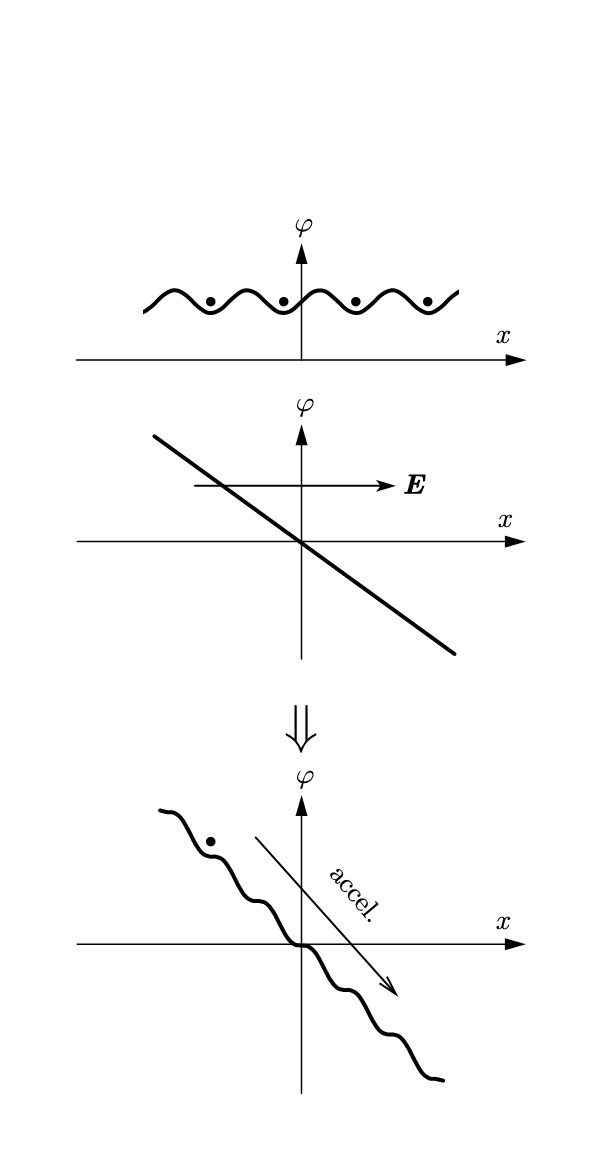
\includegraphics[width=5cm]{image/7-2-1.png}
	\caption{晶体击穿}
	\end{wrapfigure}

	\vspace{0.3cm}2. 绝缘体漏电:\,大多数非金属晶体,\,或是不含离子的液体与气体,\,原子核在晶体中都限制在点阵格子的特定位置,\,在气体,\,液体中则是可以活动的原子分子周围.\,电子分为两类,\,,一类是原子的内层电子,\,它极为稳定地存在于原子周围,\,离子晶体中的几乎完全被阴离子夺取的电子也属于这种情况.\,它们与原子核一起构成\emph{原子实}(atomic core).\,而\emph{价层电子}(valence shell electron),\,它们用来成键,\,将原子连接形成分子或者晶体,\,一般被定域在原子间的特定区域.\,所有这些电子的特点都是\emph{束缚态}(bond state).\,它们不能在介质中自由传导,\,一个电子的区域到另一个电子的区域间存在\emph{势垒}(potential barrirer),\,经典物理认为电子的动能不足以穿过这些势垒.\,但是,\,量子理论则认为电子的波函数可以通过\emph{隧道效应}(tunnelling)以小概率在不同区域间转移.\,这就为有电场的情况下电荷的平均定向移动提供了可能.\,这种现象称为\emph{漏电}(leakage).

	\vspace{0.3cm} 3. 绝缘体击穿:\,在十分高的电场下,\,原子与原子间,\,或是分子中显不同电性的部分之间的典型电压将大于阻碍电子转移的势垒.\,在晶体被击穿时此时电子在本质上可以被视为在周期性势能场与线性势能场的叠加中运动的经典粒子.\,不难看出电子不仅可以脱离单个势阱的束缚,\,还可以在这样的电场力下做持续的加速运动.\,气体液体则是在电场力作用下原子,\,分子被撕裂为离子而继续在电场力下做加速运动.\,此时碰撞就发生了:\,碰撞的结果往往是使得更多的原子分子发生电离.\,这样就会雪崩式的累积,\,固液气中的这些现象都称作\emph{雪崩击穿}(avalanche breakdown).\,尤其是气体中的放电现象在不同电流条件下分别造成\emph{汤森放电}(Townsend discharge),\,\emph{电晕放电}(corona discharge),\,\emph{辉光放电}(glow discharge),\,\emph{电弧放电}(arc discharge)的不同情况.

	\vspace{0.3cm} 4. 自然的导体:\,我们将材料区分为\emph{绝缘体}(insulator)与\emph{导体}(conductor),\,最重要的依据就是在弱场下是否天然地具有能产生电荷输运的载流子.\,所以导体就是一类事先就具有一定数密度$n$的一种或多种载流子$q$的材料,\,它们往往在有电场$\bs{E}$在场时发生位移,\,且与散射造成的形式阻力平衡,\,造成平均的匀速运动,\,即\emph{定向漂移}(directional drift).\,常见的金属以最外层的自由电子为载流子,\,半导体以热激发或掺杂形成的电子或空穴为载流子,\,电解质溶液或部分气态或液态的等离子体以阴阳离子为载流子.\,它们都是典型的导体.\,区别于前三种情况与最后的超导体.

	\vspace{0.3cm} 5. 超导体:\,低温下的很多奇异的宏观现象大大拓宽了人们对量子理论在物理学各个层次中应用的认识.\,其中很典型的一个就是\emph{超导}(superconductivity)现象.\,最早在1911年由\emph{昂内斯}({\it H. K. Onnes})在研究低温下汞的电阻率时惊人的发现在$4.2{\rm K}$下电阻率惊人地消失,\,这就是超导的发现.\,但是知道约十年后才引起足够重视.\,在$1933$年\emph{迈斯纳}({\it F. W. Meissner})才发现超导不仅仅是电阻率的消失,\,还伴随着\emph{完全抗磁性}(perfect diamagnetism):\,就好像理想导体内部无电场线,\,在超导体中交变的磁场也只能存在于表面极小的深度内(趋肤深度),\,也称迈斯纳效应.\,后来通过量子理论的蓬勃发展,\,在$1957$年提出的\emph{BCS理论}(Bardeen-Cooper-Schrieffer theory)终于解释了超导的成因,\,原来是一对\emph{库珀电子对}(Cooper pair)通过与声子(晶格振动)相互作用而造成了没有任何散射的量子模式.\,完整地解释了直到1986年所有\emph{低温超导}(low-temperatre superconductivity)的现象.\,但是随着$35{\rm K}$超导的镧钡铜氧体的发现,\,宣告人类进入\emph{高温超导}(high-temperatre superconductivity)纪元.\,新的超导材料不断被发现,\,新的理论也不断被提出,\,目前最``高温"的材料是汞钡钙铜氧体,\,超导临界温度$135{\rm}$.\,为什么有高温超导?\,高温超导的临界温度如何进一步提高?\,直到今天这也还是方兴未艾的研究领域.\,其在科研,\,科技,\,生产,\,生活方面的应用是不可估量的.

\vspace{0.5cm}

我们将把研究的范围主要放在导电的导体和不导电的绝缘体上.\,前者分析其静电平衡,\,即本章的内容;\,稳恒电流,\,下一章的内容;\,和之后章节的拟稳的一些情况.\,对于绝缘体我们本章也介绍其介电特性,\,光作为电磁波在其中的传播则放到光学中讲解.

\subsection{导体的特点}

这里说的导体,\,主要指固体形式的金属.

首先界定我们研究的问题范围:\,\emph{静电平衡}(electrostatic equilibrium)问题是一种\emph{稳态}(steady state).\,我们研究的问题由各式各样的,\,有限的块状导体${\rm C}_1,\,{\rm C}_2\cdots {\rm C}_n$构成,\,这些导体带电情况由体电荷密度$\rho$和面电荷密度$\sigma$描述.\,但是导体${\rm C}_i$上的总电荷量不一定为零:
\[Q_i=\int\limits_{{\rm C}_i}\rho \ud V+\int\limits_{\partial{\rm C}_i}\sigma \ud S\neq 0\]

这个电量$Q_i$一般也是可以在一定范围内人为控制的,\,即给导体\emph{充电}(charge).\,利用电容的性质很容易可以做到这一点.\,在为导体充电后由于电量守恒,\,其总电量就不能改变了,\,但是其电荷分布一般是未知的.


除了它们往往还有人为指定的各种点电荷$q_j$或者电荷分布$\rho(\bs{r})$存在于导体外.\,那么,\,容易想像,\,当导体外突然产生电荷分布时(如原来中和的电荷被重新分开),\,或者导体被置入电荷体系中,\,本质上就是当导体外的场环境发生改变时,\,导体内部显然不可能保持电场强度始终为零.\,只要有电场就会引起电流,\,它必然使得内部和表面的电荷分布发生改变$\dot{\rho}(t),\,\dot{\sigma}(t)\neq 0$.\,这些状态就是\emph{暂态}(transient state).\,但是只要外界的场不再变动,\,经过特征的\emph{弛豫时间}(relaxation time)后就会接近直到变成稳态.

通过以上推理,\,足以看出,\,静电平衡下,\,导体内部应当没有电场.\,这就是静电平衡理论的初始命题.\,它的初步推演泛化出以下的九宫格式的结论,\,分别讨论导体内,\,导体表面,\,导体外三处的电荷分布,\,电势分布,\,和电场分布三个特性:

\begin{table}[H]
\centering
\begin{tabular}{|c||c|c|c|}
\hline
a&a&a&a\\
\hline\hline
a&a&a&a\\
\hline
a&a&a&a\\
\hline
a&a&a&a\\
\hline
\end{tabular}
\caption{静电平衡的初级结论}
\end{table}


\section{电像法}

\section{电介质}

\section{再议静电能}
